%  Created by Branden Stone on 2015-01-15.
%  Copyright (c) 2015 Branden Stone. All rights reserved.
%--------------------------------------------------------
\documentclass{article}


%---------------------------
% Packages
%---------------------------
\usepackage{amssymb, amsmath, latexsym, amsfonts, amsthm, mathrsfs} % Standard packages that are nice to have.
\usepackage{amsrefs} % Allows for easy referencing and citations.
\usepackage{verbatim} % Needed for \begin{comment} \end{comment}.
\usepackage[text={6in,9in},centering]{geometry} % Defines the dimensions of the text body.
\usepackage[colorlinks=true]{hyperref} % Allows for use of hyperlinks.
%\usepackage[doublespacing]{setspace} % Makes the document double spaced.
\usepackage[pdftex]{graphicx} % Allows for \includegraphics
\usepackage{enumerate} % Allows for easy modification of lists

\renewcommand{\arraystretch}{1.5}

%----------------------------
% Title and Author
%----------------------------

\title{Math 390: Practice Problems for Quiz 1}
\author{}
\date{}


%----------------------------
% Main Document Body
%----------------------------

\begin{document}


%-------------------------------------------------------------
% Front Matter: This is where you can add a table of contents,
% preface, list of figures, ETC. for this template we will 
% only create a title and author name with `\maketitle'
%-------------------------------------------------------------

\maketitle

\setlength{\parindent}{0em} % Sets indentation of new paragraph
\setlength{\parskip}{1em} % Sets space between paragraphs

%-------------------------------------------------------------
% Document Body: Essentially this is where you place the 
% content of your document. To use this template, just delete
% all of the text between here and the Bibliography Section.
% Then type whatever you desire.
%-------------------------------------------------------------

\section*{Problems from the book}
\begin{center}
\begin{tabular}{lll}
	\underline{$4^{\text{th}}$ Edition} & & \underline{$5^{\text{th}}$ Edition} \\
	{ \it Section 2:} 2.3 & & { \it Section 1.1:} 1.4, 1.5 \\
	{ \it Section 5:} 5.5 & & { \it Section 2.1:} 2.6 \\
	{ \it Section 6:} 6.1, 6.2, 6.3 & & { \it Section 2.2:} 2.15, 2.16, 2.17 \\
	{ \it Section 7:} 7.1, 7.2 & & { \it Section 2.3:} 2.27, 2.28 \\
	{ \it Section 8:} 8.1, 8.4 & & { \it Section 2.4:} 2.36, 2.38 \\
	{ \it Section 11:} 11.1, 11.2 & & { \it Section 3.3:} 3.20, 3.21 \\
	{ \it Section 12:} 12.1, 12.2, 12.4 & & { \it Section 4.1:} 4.1, 4.2, 4.4
\end{tabular}
\end{center}

\section*{Additional Problems}

\begin{enumerate}
	\item Determine whether the following graphs are isomorphic. Justify your answer.
	\begin{center}
	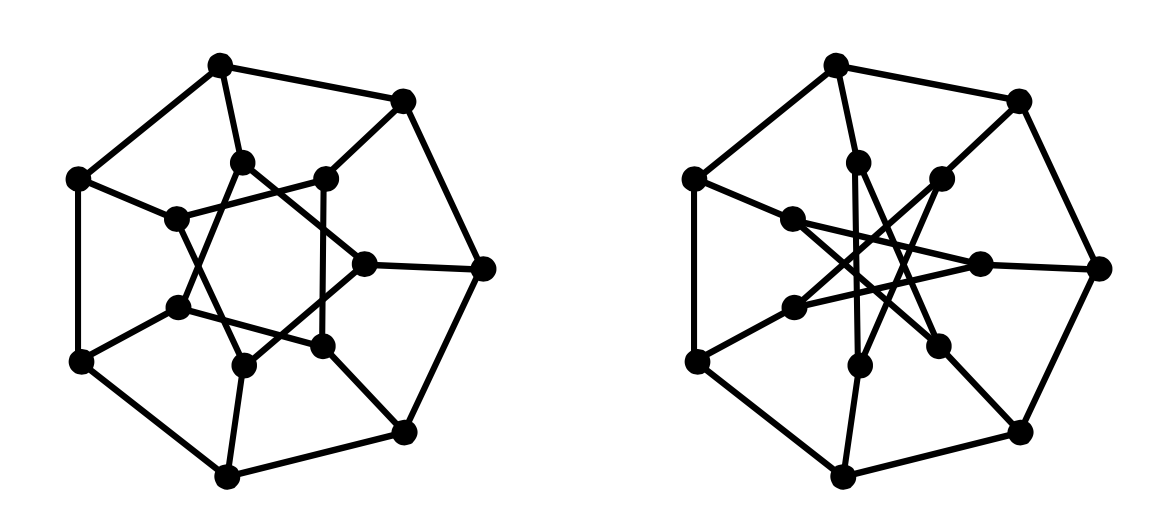
\includegraphics[width=.6\textwidth]{quiz-pic-1.png}
	\end{center}
	\item  
		\begin{enumerate}
			\item Draw all non-isomorphic simple graphs with 5 vertices and 9 edges. 
			\item Draw all non-isomorphic simple graphs with 5 vertices and 8 edges.
		\end{enumerate}

\pagebreak

	\item Consider the following graphs:
	\begin{center}
		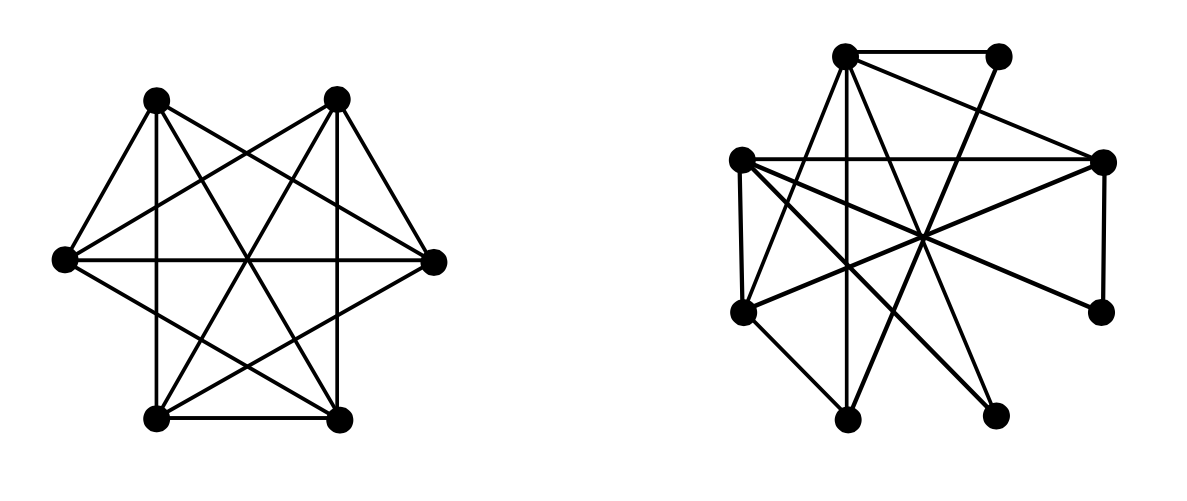
\includegraphics[width=.6\textwidth]{quiz-pic-2.png}
	\end{center}
		For each of these graphs, determine whether the graph is Eulerian. Justify your answers.

	\item Consider the following graphs:
	\begin{center}	
		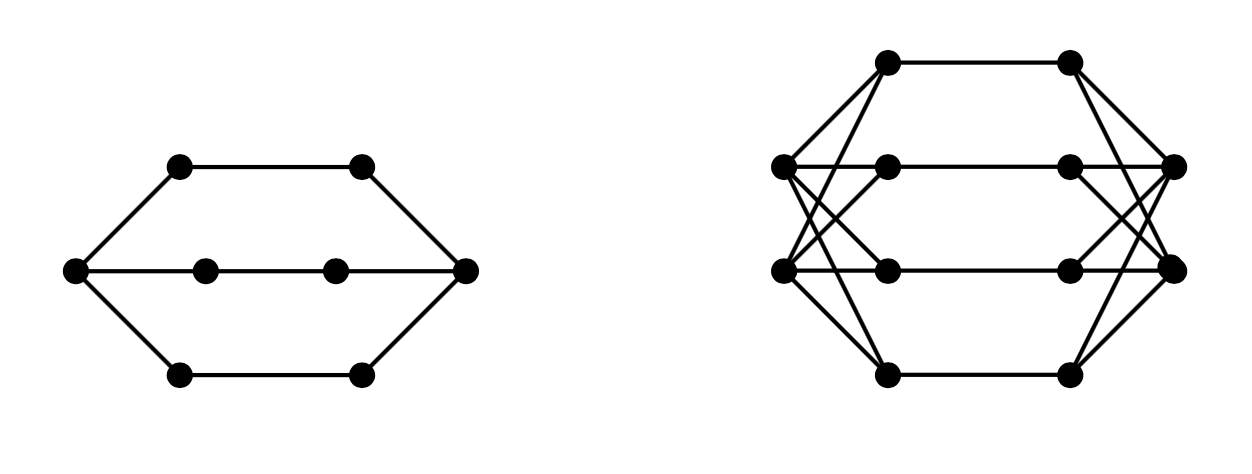
\includegraphics[width=.6\textwidth]{quiz-pic-3.png}
	\end{center}
		For each of these graphs, determine whether the graph is Hamiltonian. If the graph is Hamiltonian, indicate a Hamiltonian cycle.

	\item 
		\begin{enumerate}
			\item For which values of $n$ is $K_n$ Hamiltonian?
			\item Which complete bipartite graphs are Hamiltonian?
		\end{enumerate}

	\item Let $G$ be a weighted graph with 5 vertices $a$, $b$, $c$, $d$, $e$. For each edge, the weight is given by the following table (if two vertices do not share an edge, then the weight for those two vertices is given as $\infty$).
	\renewcommand{\arraystretch}{1.5}
			\[
			\begin{array}{c||c|c|c|c|c|}
			  & a & b & c & d & e \\
			\hline \hline
			a & 0 & 3 & 5 & 11 & 9 \\
			\hline  
			b & 3 & 0 & 3 & 9 & 8 \\
			\hline   
			c & 5 & 3 & 0 & \infty & 10 \\
			\hline 
			d & 11 & 9 & \infty & 0 & 7 \\
			\hline 
			e & 9 & 8 & 10 & 7 & 0 \\
			\hline  
			\end{array}
			\]
	Find a minimum weight spanning tree for $G$.

	\item Consider the following graph $G$:
	\begin{center}	
		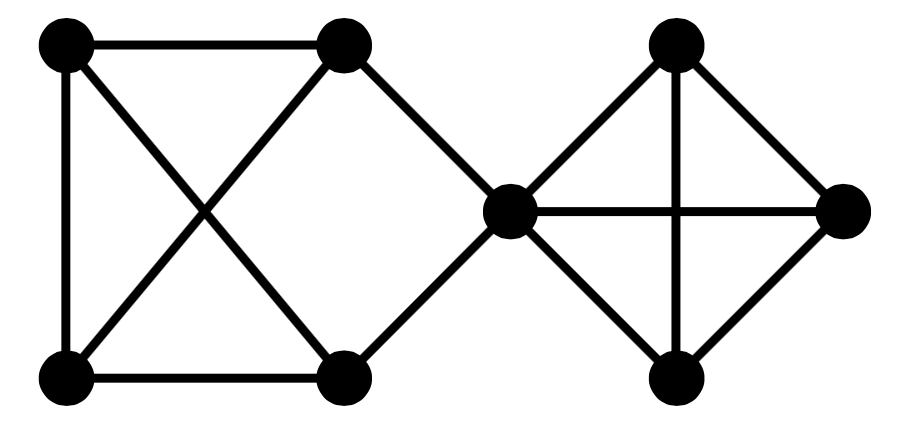
\includegraphics[width=.3\textwidth]{quiz-pic-4.png}
	\end{center}		
	Determine the connectivity $\kappa(G)$ and the edge-connectivity $\lambda(G)$ of this graph.

	\item Draw a graph $G$ with $\kappa(G)=2$ and $\lambda(G)=3$. 

	\item Suppose that $G$ is a planar graph with 20 vertices, and suppose that every vertex of $G$ has degree 3. How many edges does $G$ have? How many faces does $G$ have?

	\item Consider the following graphs:
	\begin{center}	
		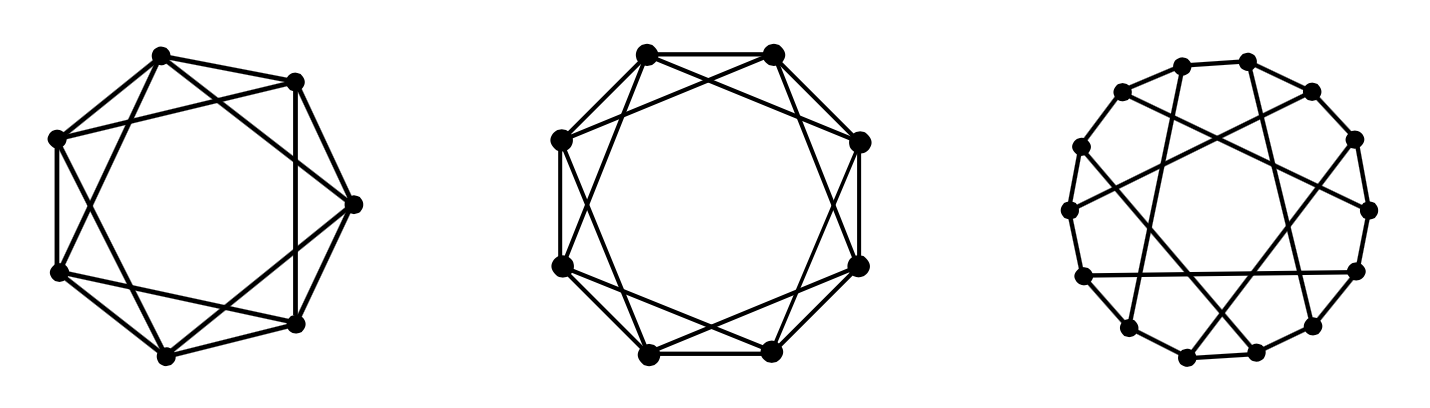
\includegraphics[width=.6\textwidth]{quiz-pic-5.png}
	\end{center}		
	For each of the above graphs, determine whether the graph is planar. Justify your answers.




\end{enumerate}


\end{document}